Hamiltonian Monte Carlo is considered a state-of-the-art sampler that efficiently explores sample space by producing large jumps to successive states with low correlation, 
but suffers the need for manual tuning of the trajectory length $\epsilon L$. 
In this chapter, we will explore improvements that adaptively adjust the trajectory length. This is achieved by means of adapting both the number of Leapfrog steps $L$ using an improved sampler called the \textit{No-U-Turn} (NUTS) sampler, and an adaptive scheme for setting the step size $\epsilon$ using a \textit{dual averaging} algorithm. We will closely follow the treatment in the original paper \cite{nuts} but adapt the notation to be consistent with the rest of this thesis.

We will start off with a discussion on how to adapt the number of Leapfrog steps using NUTS. At a high-level, NUTS starts from an initial state $(q, p)$ and simulates the Hamiltonian dynamics of the system. This is
done in the following way. Leapfrog steps are performed either forwards or backwards in time, first with a single Leapfrog step, then two Leapfrog steps, then followed by four Leapfrog steps and so on. This reiteration of the simulation is performed until the the path traced out starts to double back towards itself. The states traced out can be regarded as a \textit{balanced binary tree} $\mathcal{B}$ where
each node represents a phase-space state produced by the Leapfrog integrator during the simulation. The next state of the Markov chain is sampled at random from these nodes.  

We will end the chapter with the dual averaging scheme for adaptively setting the step size using the Leapfrog integrator. The algorithm is a modified version of a dual averaging scheme presented by Nesterov in \cite{Nesterov2009}.


\section{The No-U-Turn Sampler}
The No-U-Turn sampler generates a set of states we may regard as a balanced binary tree which we represent with the set $\mathcal{B}$. 
We shall explain the way it is built by starting from an initial point and building up the tree gradually before we generalize the procedure. An example of a trajectory generated by NUTS is shown in figure \ref{fig:nuts_trajectory}. 
The initial state $(q, p)$ is defined as the the node of the tree of depth $j = 0$. We sample a direction at random in time, either forwards ($v_0 = 1$) or backwards ($v_0 = -1$) and perform a single Leapfrog step to produce a new state $(q', p')$ using the step size $\epsilon v_0$. This state represents its own little subtree of height $j = 0$ which is to be combined with the initial node to form a tree of height $j = 1$. If $v_0 = 1$, the new node is placed as the right half of the new tree. Conversely, if $v_0 = -1$, the new node is placed as the left half of the new tree. We repeat, but this time we double the number of Leapfrog steps to $L = 2$. We randomly sample the direction once more. If forwards in time ($v_1 = 1$), we initiate the Leapfrog integrator from rightmost node of the current tree (which represents the head of the trajectory). If backwards in time ($v_1 = -1$), we feed the state of the leftmost node to the Leapfrog integrator (which represents the tail of the trajectory) and integrate backwards in time. The new states produced with the Leapfrog integrator becomes the nodes of a subtree of height $j = 1$ which will be combined with the current tree. Again, if $v_1 = 1$, we place the new subtree as the right half of the combined tree. If $v_1 = -1$, it is placed as the left half of the combined tree. 
This procedure is carried out repeatedly. We draw a direction in time at random, and perform twice as many Leapfrog steps as the prior iteration from the rightmost node if forwards in time or the leftmost node if backwards in time to extend the trajectory further. More precisely, given a tree of height $j$, 
\begin{enumerate}
    \item Sample a direction $v_j \sim \text{Uniform}(\{-1, 1\})$ in time. Set the step size in the Leapfrog integrator as $\epsilon \to \epsilon v_j$.
    \item Perform $2^j$ Leapfrog steps from the rightmost node if $v_j = 1$ or from the leftmost node if $v_j = -1$.  
    \item This generated a tree of height $j$ which is to be combined with the current tree of height $j$, producing a combined tree of height $j + 1$. If $v_j = 1$, the newly generated tree becomes the right half of the combined tree. If $v_j = -1$, it becomes the left half of the combined tree.
\end{enumerate}
From a practical perspective, we cannot apply these steps repeatedly \textit{ad-infinitum} of course. At some point, we must stop the doubling of the tree (trajectory) and select a node which will be the phase-space state to take the next place in the Markov chain. How this is solved is what we shall consider next.


\begin{figure}[h!]
    \centering
    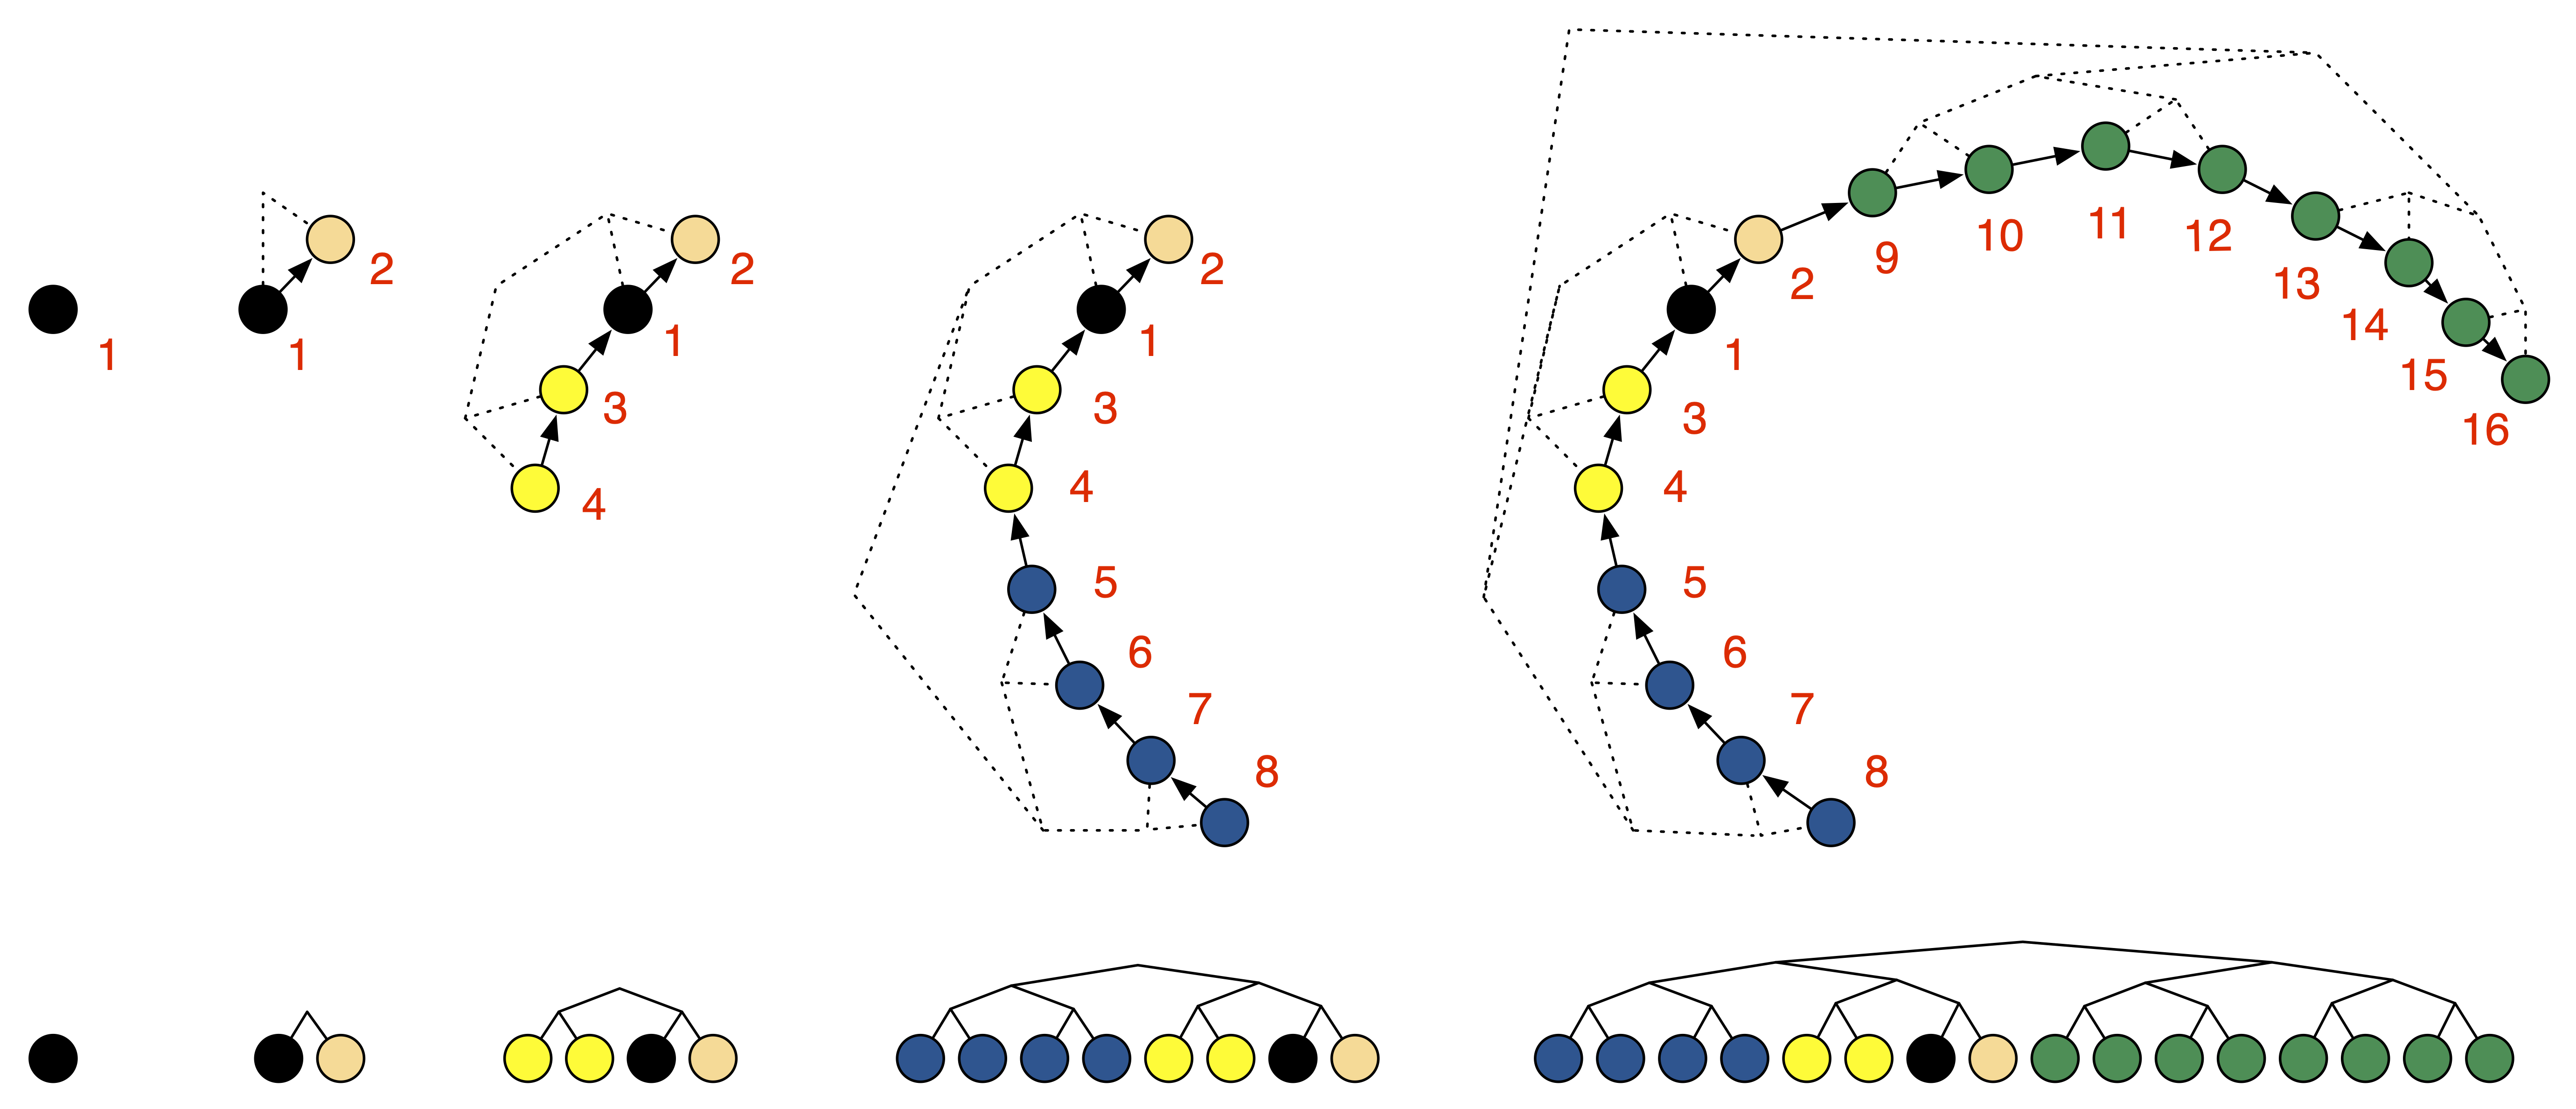
\includegraphics[scale=0.075]{figures/drawings/doubling3_with_numbering.png}
    \caption{The figure shows an example of a trajectory generated by the NUTS sampler. The balanced binary tree structure is drawn in on the trajectory as well as illustrated at the bottom. The numbering displays the order in which the states are generated by Leapfrog integration. The black node is the initial node. The first doubling is forwards in time and yields the rightmost node of the first binary tree. The second doubling is backwards in time and is initiated from the black node, yielding a new tree of height 2 where the left subtree is the new states (the yellow nodes). The next doubling is also backwards in time, and the Leapfrog integrator is initiated from the tail (the leftmost yellow node) for four Leapfrog steps generating a subtree which becomes the left half of the next tree (blue nodes). The final doubling in the figure is forwards in time with $L = 8$ Leapfrog steps are taken from the orange node (which was the leftmost leaf of the tree befoure the final doubling) which yields the green nodes. The figure is a modified version of a diagram in \cite{nuts}.}\label{fig:nuts_trajectory}
\end{figure}

\begin{comment}
    The main benefit HMC introduced over random walk Metropolis is its ability to produce large jumps in parameter space, allowing efficient exploration of the typical set. Doubling back towards other states that are already part of the trajectory is wasteful and removed the benefit HMC introduces in the first place. 
\end{comment}

\subsection{Stopping Criterion}
We seek a way to stop the doubling procedure that automatically does so when continuing is no longer beneficial from a computational standpoint.
Let us first consider a point we stressed in chapter \ref{chap:hmc}. If Hamilton's equations are solved exactly, the generated trajectory is confined to a hyperplane. Thus for an exact solution, the trajectory would at some point double back onto itself. This will likely also happen when we only approximate the solution with the Leapfrog integrator. Continuing the doubling procedure when the generated trajectory begins to double back on itself  (perform a ``U-turn''), we will revisit regions of parameter space that are already part of the binary tree, thus wasting computational resources. To avoid this, we ought to check during each doubling if such a ``U-turn'' occurs and terminate if it does. Consider an initial state $(q, p)$ taken to be the initial state and $(q', p')$ be a point produced by the Leapfrog integrator (thus treated as a function of time). Then the change in the Euclidean distance between the positions are
\begin{equation}\label{eq:change_in_distance}
    \dv{t}\frac{\norm{q' - q}_2^2}{2} = (q' - q)^T \dv{t}  (q' - q) = (q' - q)^Tp',
\end{equation}










\subsection{Generation of States and the Stopping Criterion}
Up until this point, we have not yet described precisely how the states in $\mathcal{B}$ are generated,
nor why and when to stop its generation. As we briefly described in the introduction to this chapter, 
NUTS computes trajectories in phase-space until the trajectory starts to double back on itself. First running one Leapfrog step,
then two Leapfrog steps, then four Leapfrog steps and so on. Each such step is run either forwards or backwards in ficticious time, chosen at random.
If the direction is forwards, it starts from the state at the \textit{head} of the total generated trajectory. If the direction is backwards in time, it starts from the state corresponding to the \text{tail} of the trajectory.
The successive state produced by the Leapfrog integrator at each such step is collected and stored. This generates a collection of states which we represent with $\mathcal{B}$. 




The No-U-Turn sampler augments standard HMC by introduction of a \textit{slice variable} $u$ which is sampled according to
\begin{equation}
    u \sim p(u|q, p) = \text{Uniform}\left(u; \left[0, \exp\left\{-H(q, p)\right\}\right]\right).
\end{equation} 
A slice variable impose a condition, in this case on $(q, p)$, that require that any valid state $(q, p)$ must lie within the slice defined by $u$. This imply a conditional distribution on $(q, p)$ given $u$
\begin{equation}
    p(q, p|u) = \text{Uniform}\left( q, p; \left\{q, p \bigg| \exp\left\{-H(q, p)\right\} \geq u \right\} \right).
\end{equation}
The distribution simply states that any state $(q, p)$ that lies in the set such that $\exp\{-H(q, p)\} \geq u$ is valid and is equally likely.
Consequentially, we have the joint distribution 
\begin{equation}
    p(q, p, u) \propto \mathbb{I}\left[u \in \left[0, \exp\left\{-H(q, p)\right\}\right]\right],
\end{equation}
where $\mathbb{I}[\cdot]$ evaluates to $1$ if its argument is true and $0$ otherwise. 
Integrating with respect to $u$ yields the marginal distribution
over phase-space
\begin{equation}
    p(q, p) = \int p(q, p, u) \dd u \propto \int_0^{\exp\left\{-H(q, p)\right\}}\dd u = \exp\left\{-H(q, p)\right\}.
\end{equation}
which is the target distribution we use in standard HMC.